
\documentclass{jfm}

\begin{document}

\newtheorem{lemma}{Lemma}
\newtheorem{corollary}{Corollary}

%% \Rey, \Pran and \Pen are defined by template
\newcommand\Sch{\mbox{\textit{Sc}}} % Prandtl number, cf TeX's \Pr product
\shorttitle{Nonlinear Goldreich-Schubert-Fricke} %for header on odd pages
\shortauthor{J. S. Oishi et al} %for header on even pages

\title{GSF Simulations}

\author
 {
 Jeffrey S. Oishi\aff{1}
  \corresp{\email{oishij@farmingdale.edu}},
  Keaton Burns\aff{2},
  Daniel Lecoanet\aff{3},
  Geoffrey Vasil\aff{4},
  Ben Brown\aff{5},
  Susan E. Clark\aff{6}
  }

\affiliation
{
\aff{1}
Department of Physics, Farmingdale State College, Farmingdale, NY 11735
\aff{2}
Department of Physics, Massachussetts Institute of Technology, Cambridge, MA 02139
\aff{3}
Department of Astronomy, University of California, Berkeley, Berkeley, CA 94720
\aff{4}
School of Mathematics \& Statistics, University of Sydney, NSW 2006, Australia
\aff{5}
Laboratory for Atmospheric \& Space Physics and Department of Astrophysical \& Planetary Sciences, University of Colorado, Boulder, Colorado 80309, USA
\aff{6}
Department of Astronomy, Columbia University, New York, NY 10024

}

\maketitle

\begin{abstract}
Dedalus simulations of the GSF!
\end{abstract}

\section{Introduction}
\label{sec:intro}
The Goldreich-Schubert-Fricke instability \citep{1967ApJ...150..571G}

\section{The Model}
\label{sec:model}

In order to study the GSF, we use a simplified equation set designed
to capture the relevant physics in a simple, controlled numerical
experient. We use the Spiegel-Veronis Boussinesq approximation for
radially stratified, compressible, perfect gasses,
\begin{equation}
  \label{eq:continuity}
  \mathbf{\nabla \cdot v} = 0,
\end{equation}
\begin{equation}
  \label{eq:momentum}
  \frac{\partial \mathbf{v}}{\partial t} + \mathbf{v \cdot \nabla v} = -\frac{\mathbf{\nabla} p}{\rho_m} + g \frac{T'}{T_m}\mathbf{\hat{r}} + \nu \nabla^2 \mathbf{v},
\end{equation}
and
\begin{equation}
  \label{eq:temp}
  \frac{\partial T'}{\partial t} + \mathbf{v \cdot \nabla} T' + u \left[\frac{d T_m}{dr} - \left(\frac{d T_m}{dr}\right)_{ad}\right] = \chi \nabla^2 T'.
\end{equation}
In the above equations, we have separated the variables into mean and
fluctuating quantities, e.g. $T(r, \theta, z) = T_m(r) + T'(r, \theta, z)$, and $(d T_m/dr)_{ad}$ is the
adiabatic background gradient.

We can simplify these equations by noting that the Brunt-V\"ais\"al\"a frequency can be written as
\begin{equation}
  \label{eq:brunt}
  N^2 = \frac{g}{T}\left[\frac{d T}{dr} - \left(\frac{d T}{dr}\right)_{ad}\right],
\end{equation}
and by creating a new variable $\Theta \equiv g T'/T_m$. Equations~(\ref{eq:momentum}) and (\ref{eq:temp}) can then be rewritten as 
\begin{equation}
  \label{eq:final_momentum}
  \frac{\partial \mathbf{v}}{\partial t} + \mathbf{v \cdot \nabla v} = -\frac{\mathbf{\nabla} p}{\rho_m} + g \Theta \mathbf{\hat{r}} + \nu \nabla^2 \mathbf{v},
\end{equation}
and
\begin{equation}
  \label{eq:final_temp}
  \frac{\partial \Theta}{\partial t} + \mathbf{v \cdot \nabla} \Theta + N^2 u = \chi \nabla^2 \Theta.
\end{equation}

In addition to dynamical variables, we track the evolution of a dye concentration field $c$, which follows 
\begin{equation}
  \label{eq:dye}
  \frac{\partial c}{\partial t} + \mathbf{\nabla \cdot} (c \mathbf{u}) = \nu_{dye} \nabla^2 c.
\end{equation}

In all calculations, the Schmidt number $\Sch \equiv \nu/\nu_{dye} = 1$.

The exact equations as entered in our numerical framework Dedalus (see
section~\ref{sec:numerical} for details) can be found in
Appendix~\ref{sec:appendix_dedalus}.

We consider these equations in a cylindrical Taylor-Couette (TC) geometry
periodic in the axial ($z$) direction, with impenetrable, no-slip
walls in $r$. The equations are non-dimensionalized in terms of the
gap width $[L] = \delta = R_2 -R_1$, where the subscripts 1 and 2
refer to the inner and outer cylinders, respectively. We measure
velocities in units of the inner cylinder velocity,
$[V] = R_1 \Omega_1$, with $\Omega_1$ the inner cylinder rotation
rate. 

We define $\Rey = R_1 \Omega_1 \delta/\nu$, so in our non-dimensional
formulation, $\Rey = 1/\nu$. It is also helpful to consider the epicyclic frequency, 
\begin{equation}
  \label{eq:epicyclic_freq}
\kappa^2 = \frac{1}{r^3}\frac{d (r^2 \Omega_0)^2}{dr}
\end{equation}
of the background Couette flow, $\Omega_0 = A + B/r^2$. $A$ and $B$
are computed from the parameters $\eta = R_1/R_2$ and
$\mu = \Omega_2/\Omega_1$, characterizing the geometry and
differential rotation of the system. For Couette flow, we can write 
\begin{equation}
  \label{eq:kappa_couette}
  \kappa^2 = - 4 \Omega_1^2 \eta^2
  \frac{(1-\mu)(1-\mu/\eta^2)}{(1-\eta^2)^2}
  \left[\frac{R_2^2}{r^2} -\frac{(1-\mu/\eta^2)}{(1-\mu)} \right].
\end{equation}

\section{Linear Analysis}
\label{sec:linear}
The linear properties of the GSF are well documented in GS67 and
F68. Here, we summarize their dispersion relation 

\section{Numerical Methods}
\label{sec:numerical}
We use the Dedalus framework (available for download at
http://dedalus-project.org). 

We initialize our simulations with Couette flow in $v$ and
low-amplitude Gaussian white noise in $\Theta$ with a sharp cutoff at
$k_r/k_{max} > 0.3$ and $k_z/k_{max} > 0.3$. The cutoff prevents
unresolved oscillations from polluting the calculation.

\section{Results}
\label{sec:results}

First, we consider a fiducial case, with $\Rey = 10^6$,
$\Pran = 10^{-2}$, $\mu = 0.9425$, $N^2 = 15.5$, and $\eta = 0.99$. The
fiducial run has resolution $256^2$. 

\begin{figure}
  \centering
  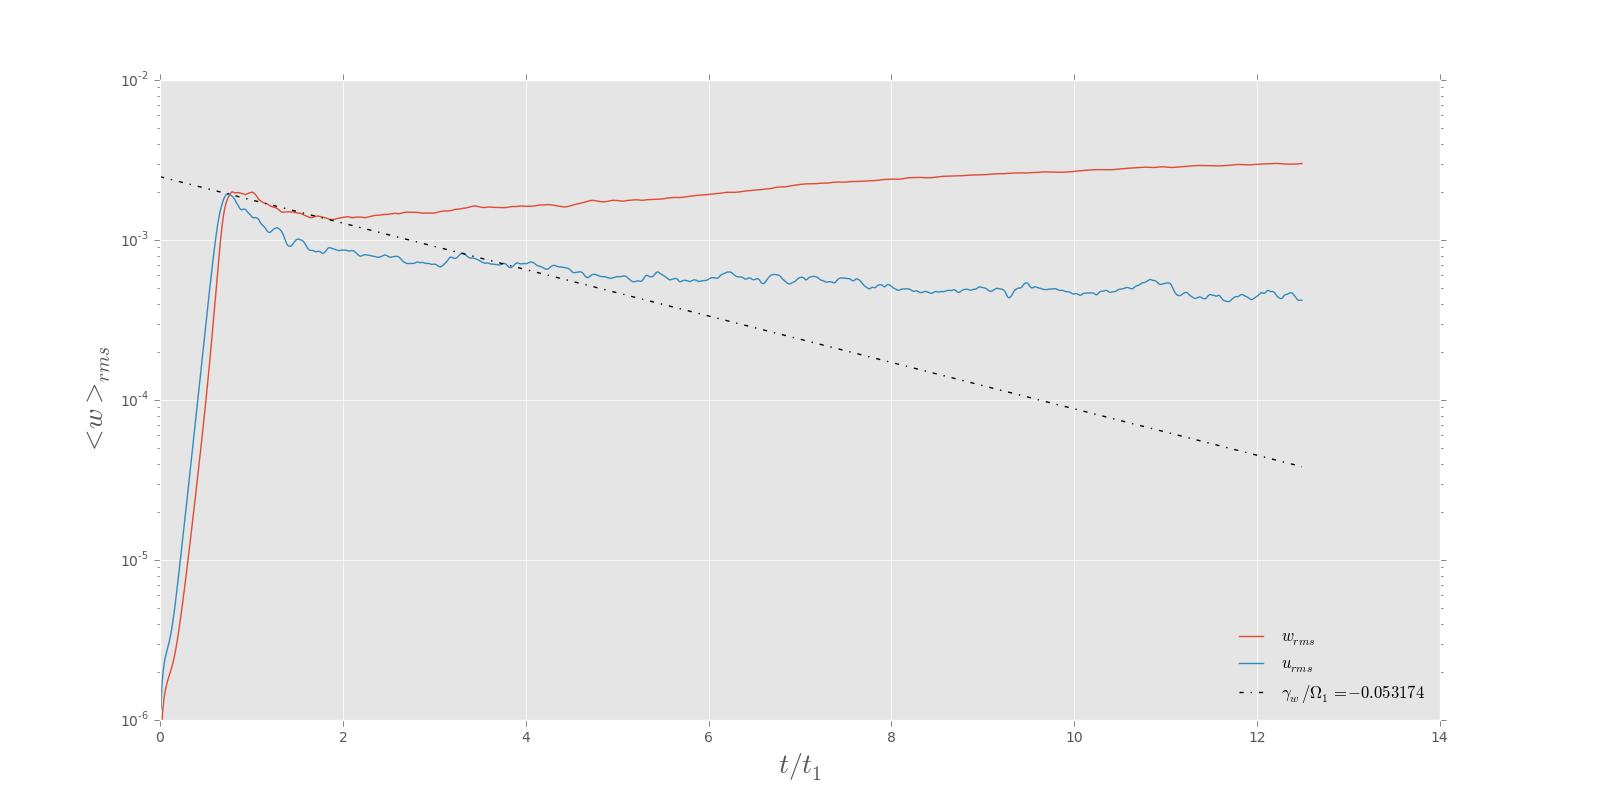
\includegraphics[width=\textwidth]{../../figs/rms_vel_re1.00e+06_mu9.43e-01_eta9.90e-01_Pr1.00e-02_N21.55e+01_nz256.png}
  \caption{RMS velocities $<u>_{rms}$ and $<w>_{rms}$ as a function of time for the fidicial run. }
  \label{fig:fid_energies}
\end{figure}

\begin{figure}
  \centering
  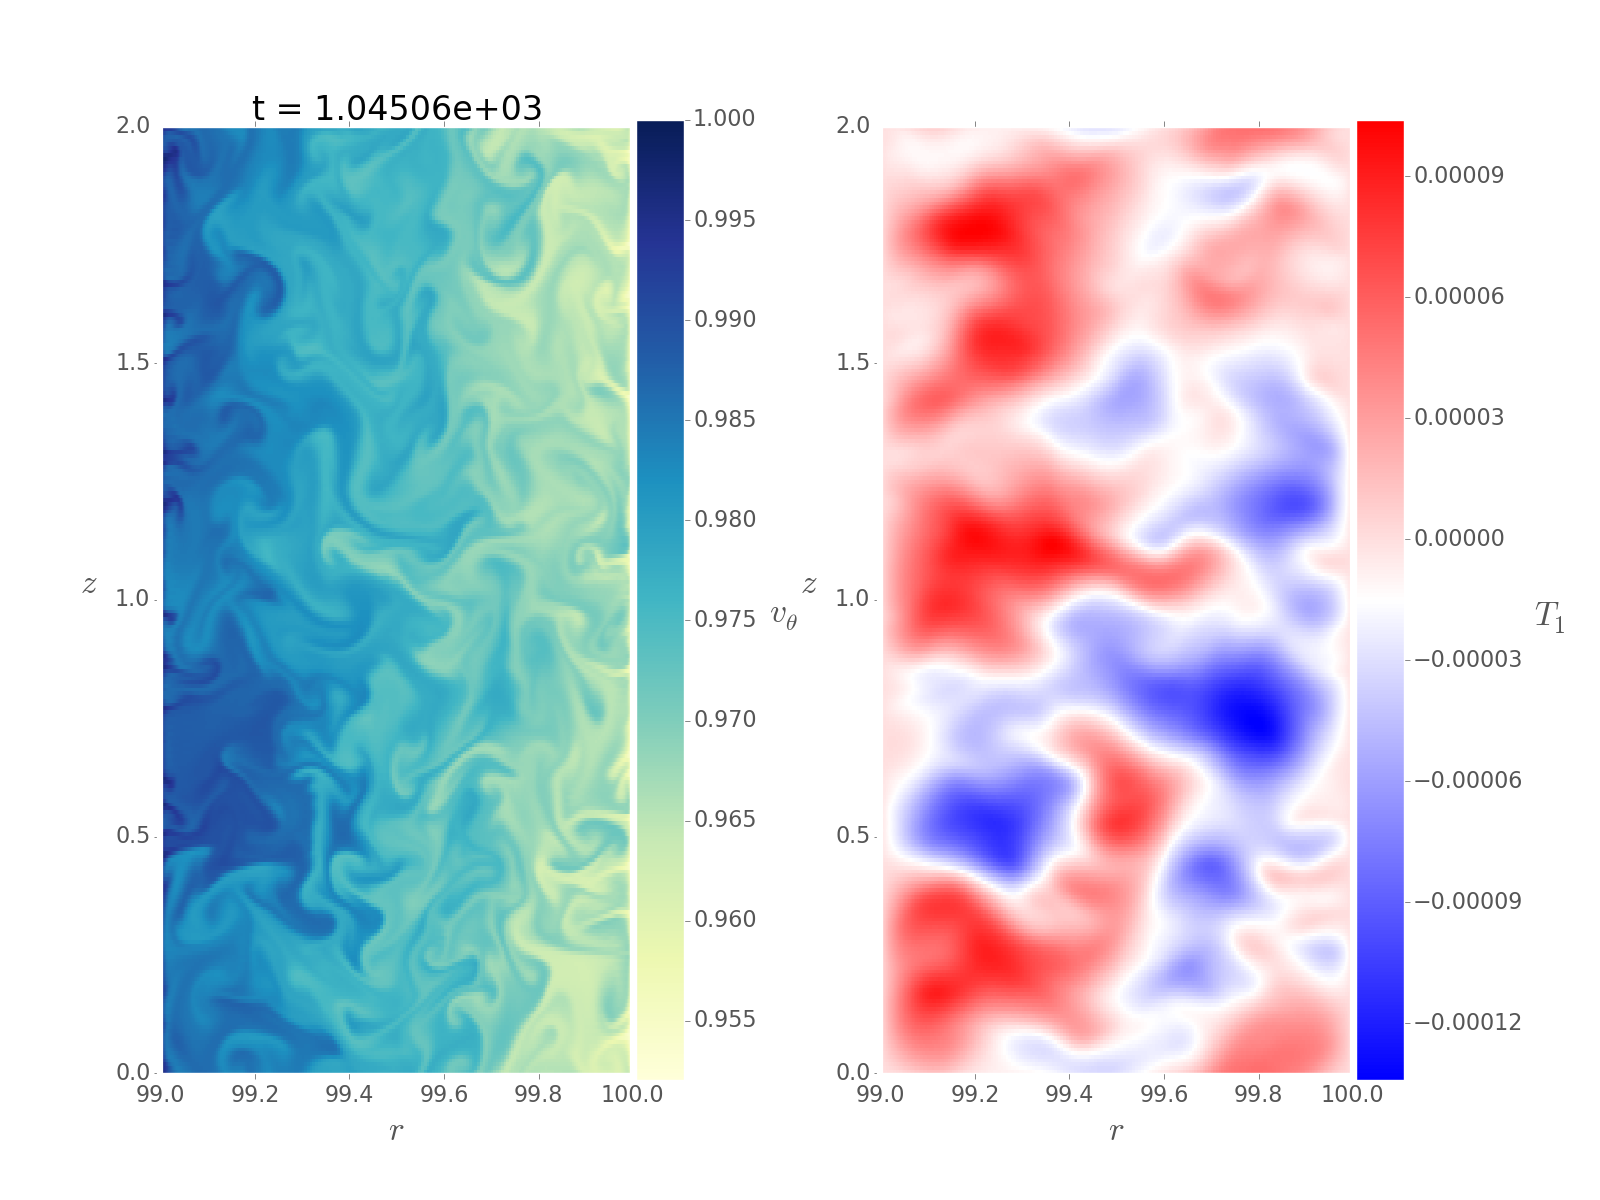
\includegraphics[width=\textwidth]{../../figs/vel_frame_0155_re1.00e+06_mu9.43e-01_eta9.90e-01_Pr1.00e-02_N21.55e+01_nz256.png}
  \caption{$v$ and $\Theta$ in the fiducial run after saturation but before the development of the mean flow.}
  \label{fig:fiducial_slice_early}
\end{figure}
\subsection{Mixing}
\label{sec:mixing}

\subsection{Mean Flow}
\label{sec:meanflow}


We thank Mordecai-Mark Mac Low and Alex Hubbard for useful
discussions. JSO is supported by a Provost's Research Fellowship from
Farmingdale State College.
\appendix
\section{Exact Dedalus Equations}
\label{sec:appendix_dedalus}
The exact equations entered in Dedalus are 

\bibliography{library_filtered2}
\bibliographystyle{jfm}

\end{document}
